\chapter{Análise Bibliográfica sobre Blockchain na Economia Global, por Fernando Ferreira Cordeiro\label{chap:bibliometria:FernandoCordeiro}}

\section{Planejamento do estudo}

O \textit{blockchain} é um sistema de registro de informações, embora seja distinto de um banco de dados típico na forma como armazena informações; as informações em um \textit{blockchain} são armazenadas de tal forma que torna difícil ou impossível alterar, hackear ou enganar o sistema. 
Com essa tecnologia o mercado global encontrou uma capacidade de digitalizar com segurança muitas operações atuais em economia e finanças, e serviços jurídicos e governamentais.

\textit{Blockchain} está revolucionando rapidamente a economia mundial. O efeito potencial da tecnologia blockchain  na sociedade e no economia global são extremamente importantes, pois prometem sempre ter um impacto otimista sobre o futuro.

Tendo como base o exposto acima, os pontos principais aqui abordados serão:
\begin{itemize}
    \item Onde a tecnologia de Blockchain é aplicada na economia?
    \item Quais novas oportunidades vieram com o Blockchain?
    \item Como o Blockchain está entralassado com economias emergentes?
\end{itemize}

\subsection{Uso do Bibliometrix e Biblioshiny}
Serão usadas a ferramenta e o \textit{workflow} proposto pelos autores do pacote Bibliometrix, conforme indica a figura ~\ref{fig:bibliometrix:workflow}.

\subsection{Limitações} O exercício relatado não possui uma base de dados extensa, um pouco acima do mínimo exigido. E o mesmo se da ao tempo aplicada para a mesma, por ser um atividade inaugural no assunto, não é esperada uma análise profunda.


\section{Coleta de dados}

A coleta de dados feita usando a base do WoS (Web of Science) no dia 09 de Fevereiro de 2022, acessado por meio do Portal de Periódicos da CAPES

Foi usada a \textit{query} de busca ilustrada na listagem:

\lstinputlisting[numbers=left,basicstyle=\normalsize\ttfamily,caption={Query de busca para \textit{Blockchain} na \textit{Economia Global}}]
{experiments/FernandoCordeiro/AnaliseBibliometrica/Blockchain/query.txt}

\subsection{Explicação para os termos de busca usados\label{sec:FernandoCordeiro:query}}

A busca consistiu de 2 cláusulas conectadas por uma operação AND para trazer informações sobre a tecnologia de \textit{blockchain}, aplicadas à busca por tópico.

O termo \textit{blockchain} (linha 1) foi utilizado na primeira cláusula da \query\ para recuperar artigos em seu título, palavras-chave e resumo, termos relacionados a \textit{blockchain}. 

Os termos \textit{global}, \textit{economy} e \textit{market} (linhas 3 - 6)foram usados na conjunção com o primeiro para recuperar trabalhos que apenas estejam relacionados a economia ou ao mercado global.

Foram obtidos 285 registros com a \textit{query} utilizada. Na exportação, foi utilizado o formato de arquivo de texto sem formatação, com os 29 campos disponíveis.

\subsection{Registros recuperados}

Foram utilizadas as opções \textit{Exportar registros para arquivo de texto sem formatação} e \textit{export full record / Gravar Conteúdo: Seleção personalizada, com todos os 29 campos disponíveis, inclusive referências citadas} no WoS, para que as citações também fosse usadas em análises da citações (estrutura intelectual do conhecimento). 
Os 285 registros recuperados em um único bloco de até 1.000 registros.

\section{Análise dos dados}

\subsection{Filtragem de registros}

Antes da análise, foi aplicado filtros sobre o \dataset\ inicial, para remover os registros indesejados. Foi mantido apenas os registros de artigos públicados em revistas científicas (supondo que o conhecimento de maior qualidade a respeito do tema está nas revistas, afinal é o método padrão de publicação científica).  Após a filtragem, foram mantidos 149 registros  no \dataset\ para a análise.

\subsection{Análise descritiva do \textit{dataset} }

A análise bibliométrica descritiva faz uma descrição inicial do \textit{dataset}, utilizado a função \texttt{biblioAnalysis} do Bibliometrix, para realizar diversos cálculos para levantar as taxas apresentadas

As informações mais gerais sobre o \textit{dataset} são as seguintes:
\begin{description}
    \item [\textit{Timespan}] Os artigos filtrados foram publicados entre 2017 e 2022, dado a novidade da tecnologia, é esperado publicações recentes.
    \item [\textit{Sources (Journals, Books, etc)}] São 122 fontes de informação que publicaram os artigos recuperados no \textit{dataset}. Logo, a média de publicações por \textit{scientific journal} é de $1.033/537=1,9$ artigos.
    \item [\textit{Average years from publication}] A média do tempo de publicação dos artigos no \textit{dataset} é de 2,11 anos.
    \item [\textit{Average citations per documents}] Cada artigo no \textit{dataset} foi citado, em média 8,664 vezes.
    \item [\textit{Average citations per year per doc}] Após publicado, cada um dos artigos foi citado, em média, 2,551 vezes por ano.
    \item [\textit{References}] O \textit{dataset} contém 8.466 referências citadas.
    \item [\textit{Keywords Plus (ID)}] 282 distintas palavras-chave do tipo Keywords Plus (ID) foram encontradas no \textit{dataset}.
    \item [\textit{Author's Keywords (DE)}] 663 distintas palavras-chave indicadas pelos autores foram encontradas no \textit{dataset} .
    \item [\textit{Authors}] 462 distintos nomes de autores foram encontrados no \textit{dataset} .
    \item [\textit{Author Appearances}] Os 462 distintos autores foram encontrados 474 vezes, como autores de artigos.
    \item [\textit{Authors of single-authored documents}] Dentre os 462 distintos autores encontrados, 34 deles editaram artigos individualmente, isso é, sem co-autores.
    \item [\textit{Authors of multi-authored documents}] Dentre os 462 distintos autores encontrados, 428 deles editaram artigos com um ou mais co-autores"
    \item [\textit{Single-authored documents}] Dentre os 149 documentos presentes no \textit{dataset}, 34 foram escritos por um único autor, e os restantes foram elaborados em co-autoria.
    \item [\textit{Documents per Author}] Dentre os 462 distintos autores, tem-se uma média 0,323 artigos publicados por autor.
    \item [\textit{Authors per Document}] Cada um dos 149 documentos presentes no \textit{dataset} foi autorado com 3,1 autores em média.
    \item [\textit{Co-Authors per Documents}] As 474 aparições de autores (``Author Appearances''), distribue-se em média 3,18 vezes para os 149 artigos do \textit{dataset}.
    \item [\textit{Collaboration Index}] Os 462 autores que editaram artigos com um ou mais co-autores, colaboraram em media 3,72 vezes para editar os 149 artigos elaborados em co-autoria, gerando, assim, um índice de colaboração 4,33. 
\end{description}

\subsection{Evolução da Produção Científica}

\begin{figure}
    \centering
    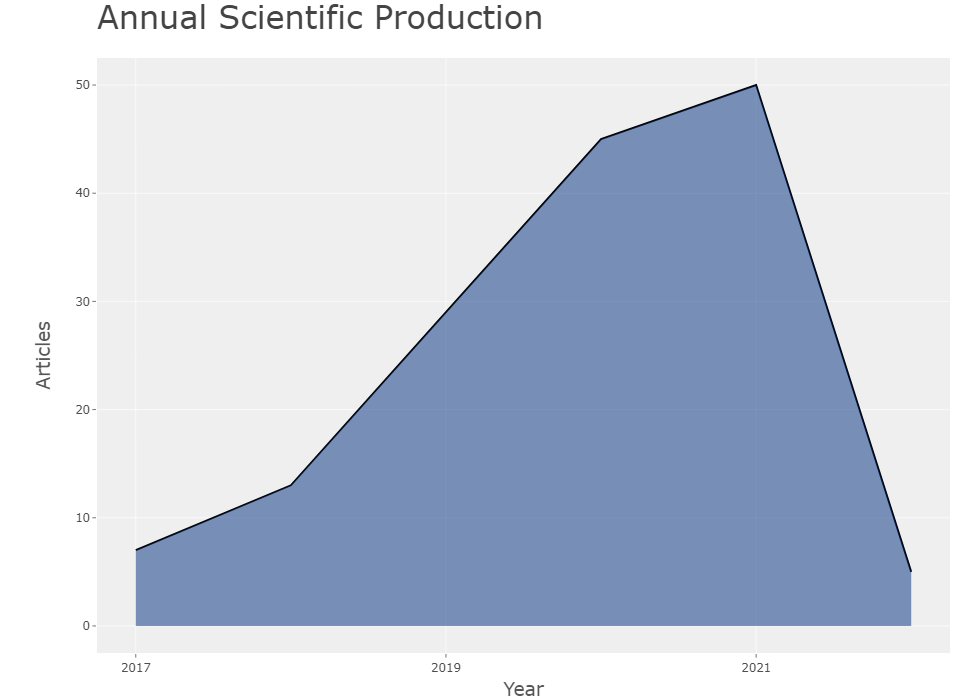
\includegraphics[width=1\textwidth]{experiments/FernandoCordeiro/AnaliseBibliometrica/Blockchain/annual_plot.png}
    \caption{Evolução da produção científica no \textit{dataset}}
    \label{fig:evol:anual:BLOCKCHAIN@FernandoCordeiro}
\end{figure}

A figura \ref{fig:evol:anual:BLOCKCHAIN@FernandoCordeiro} representa a evolução em produção científica mundial a respeito do tema, de acordo com o \textit{dataset}. Houve um crescimento a notável a partir do ano de 2018, atingindo o pico em 2021. 

O \textit{Annual Growth Rate} do \textit{dataset} é de -6,51\%, um crescimento negativo devido a baixa produtividade científica os anos de 2021 e 2022.

\subsection{Interpretação do Crescimento} 
A taxa de crescimento do \textit{dataset} demonstra que o tema tem chamado muita atenção no seu começo, provavelmente devido principalmente ao mercado de criptomoedas.

\subsection{Evolução das Citações}

\begin{figure}
    \centering
    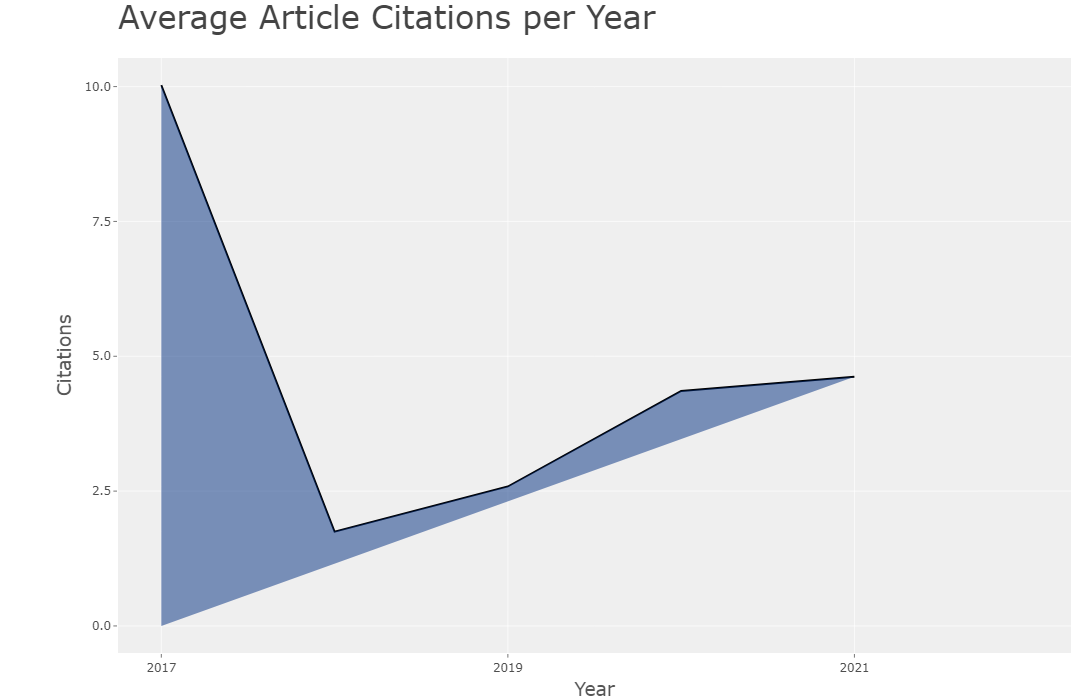
\includegraphics[angle=0,width=1\textwidth]{experiments/FernandoCordeiro/AnaliseBibliometrica/Blockchain/citations_year_plot.png}
    \caption{Evolução das citações ao \textit{dataset}.}
    \label{fig:evol:anual:citacoes:BLOCKCHAIN@FernandoCordeiro}
\end{figure}

A figura \ref{fig:evol:anual:citacoes:BLOCKCHAIN@FernandoCordeiro} apresenta a evolução da média de citações aos artigos do \textit{dataset}. Não há muita estabilidade na média anual de citações, tendo uma grande vale no período analisado.

\subsection{Interpretação das Citações}
Embora a taxa de crescimento de publicações anuais seja alta, ainda há instabilidade no que diz respeito a média de citações. Demonstrando que o tema ainda é um tanto prematuro, necessitando de mais atenção pelos cientistas.

\subsection{\textit{Three-Field Plots (Sankey diagram)}}

As \textit{Three-Field Plots (Sankey diagram)} (plotagens do tipo ``Três Campos'') correlacionam três conjuntos de atributos em busca das afinidades encontradas no \textit{dataset}. Assim, são demonstrados os principais fluxos entre diferentes conjuntos.

\begin{figure}
    \centering
    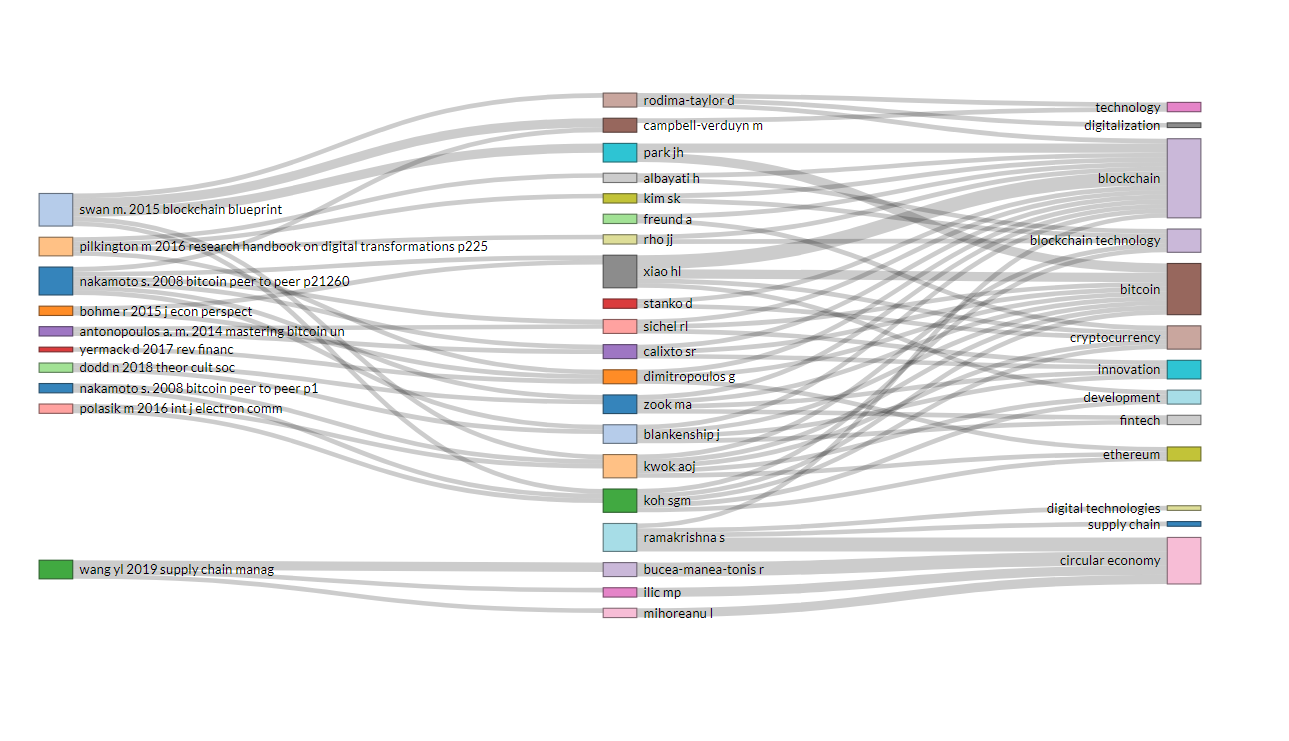
\includegraphics[width=1\textwidth]{experiments/FernandoCordeiro/AnaliseBibliometrica/Blockchain/Three-Fields_Plot.png}
    \caption{Plotagem ``Três Campos'' (Sankey plot) do \textit{dataset}: 20 Autores, 20 Citações e 20 Palavras-Chave mais proeminentes.}
    \label{fig:BLOCKCHAIN@FernandoCordeiro:ThreeFieldPlot}
\end{figure}

A figura \ref{fig:BLOCKCHAIN@FernandoCordeiro:ThreeFieldPlot} apresenta a plotagem do tipo ``Três Campos'' realizada no \textit{dataset}, vinculando, ao centro, os 20 Autores mais proeminentes (AU), à esquerda, as 20 Citações mais frequentes (CR - Cited Records), e à direita, as 20 Palavras-Chave mais frequentes empregadas pelos autores.

\subsection{Interpretação da figura \ref{fig:BLOCKCHAIN@FernandoCordeiro:ThreeFieldPlot}}
Os 20 autores mais relevantes apresentados na plotagem são, aparentemente, de origem oriental. O que sugere o avanço e a preocupação do oriente a respeito do tema analisado, em principal sore bitcoin e economia circular.

É possível observar nas palavras-chave que há bastante interesse no mercado de criptomoedas, apresentam-se os termos \textbf{bitcoin}, \textbf{cryptocurrency}, \textbf{blockchain technology} e \textbf{circular economy}. Os resultados sugerem que há interesse no mercado de cripto moedas e como ela movimenta o mercado global.

\section{Refinamento da Coleta de Dados}

Após a análise do \textit{dataset}, foi possível notar que os artigos estão relacionados ao tema, devido ao baixo número de documentos. A observação indica que não a necessidade de uma nova busca, visando a exclusão de artigos não relacionados ao desenvolvimento de \textit{blockchain} na economia global.

\begin{figure}[htp]
    \centering
    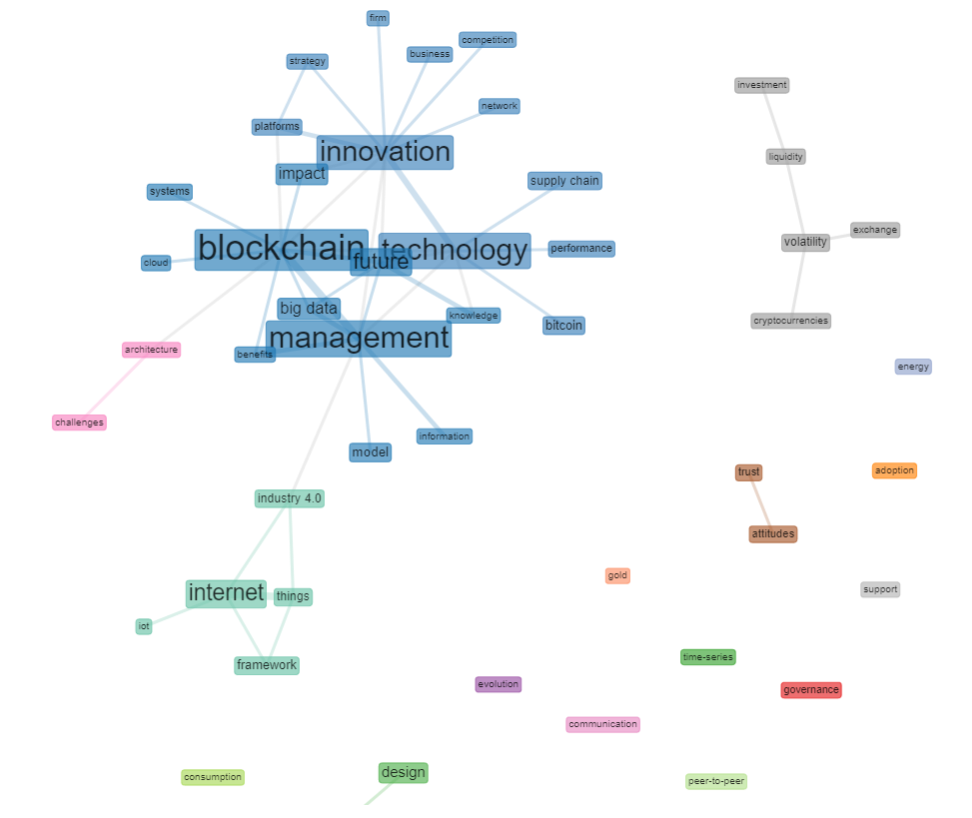
\includegraphics[width=0.6\textwidth]{experiments/FernandoCordeiro/AnaliseBibliometrica/Blockchain/co-ocurrence.png}
    \caption{Rede de co-ocorrência de palavras aplicada ao \textit{dataset}.}
    \label{fig:BLOCKCHAIN@FernandoCordeiro:redecoocorrencia}
\end{figure}

O conjunto das palavras-chave que refletia e o tema ficou evidente na análise da estrutura intelectual do conhecimento, do tipo \textbf{Rede de Co-ocorrências de Palavras-chave}.

As seguintes 20 palavras principais foram identificadas nesse \textit{cluster}:
blockchain,
management,
model,
future,
big data,
supply chain,
technology,
innovation,
platforms,
bitcoin,
impact,
performance,
design,
trust,
attitudes,
volatility,
framework,
internet,
things,
industry 4.0.

\section{Nova Análise dos Dados}
    Como a análise previa dos dados se mostraram satisfatorias para a proposta da atividade apresentada, no qual todas as palavras-chave se relacionaram corretamento com o tema \textit{Blockchain na Economia Global}, não se mostrou necessidade da criação de uma nova \query\ para recuperar uma nova coleção de dados. Sendo assim a \query\ original foi mantida e não será feito uma nova análise. 

\subsection{Análise descritiva do \textit{dataset} refinado}

\begin{table}[]
    \centering
\csvautotabular[separator=semicolon
%,filter not strcmp={\csvcolii}{}
]{experiments/FernandoCordeiro/AnaliseBibliometrica/Blockchain/main_information.csv}
    \caption{Principais dados descritivos do dataset.}
    \label{tab:BLOCKCHAIN:Main}
\end{table}

Logo, de acordo com a tabela \ref{tab:BLOCKCHAIN:Main}, é possível notar que entre 2017 e 2022 houveram 149 artigos publicados em 122 revistas diferentes.